%%
% The BIThesis Template for Bachelor Graduation Thesis
%
% 北京理工大学毕业设计(论文)第一章节 —— 使用 XeLaTeX 编译
%
% Copyright 2020 Spencer Woo
%
% This work may be distributed and/or modified under the
% conditions of the LaTeX Project Public License, either version 1.3
% of this license or (at your option) any later version.
% The latest version of this license is in
%   http://www.latex-project.org/lppl.txt
% and version 1.3 or later is part of all distributions of LaTeX
% version 2005/12/01 or later.
%
% This work has the LPPL maintenance status maintained'.
%
% The Current Maintainer of this work is Spencer Woo.
%
% 第五章节
\chapter{树状区块链应用和性能测试}
本章中,将地图信息存储与展现成功应用于树状区块链上,在此基础上,将李玮琪的车辆位置验证与信誉评估系统\cite{lposition}应用于当前地图存储与显示方法,取得不错的成效。最后,测试了树状区块链与传统区块链存储性能的区别,并得到相关数据结果。

\section{基于区块链地图数据的车辆位置验证与信誉评估系统}
本小节将地图存储与展现工作移植到树状区块链上,并上传北京地图数据,实现了地图展现,在此基础上,复现了李玮琪车辆位置验证与信誉评估\cite{lposition},验证了树状区块链相关功能的正确性。

\subsection{移植地图存储与展现}
首先,根据第一章复现树状区块链的方法建立树状区块链私有链,将地图存储合约进行部署,然后通过JS脚本将北京市地图数据上传,同时进行区域绑定工作。最后,通过GeoHashTile前端将请求获得的数据处理并展现, 结果展示,如图\ref{地图数据上传全图},\ref{局部放大图}。
\begin{figure}[!htb]
    \centering
    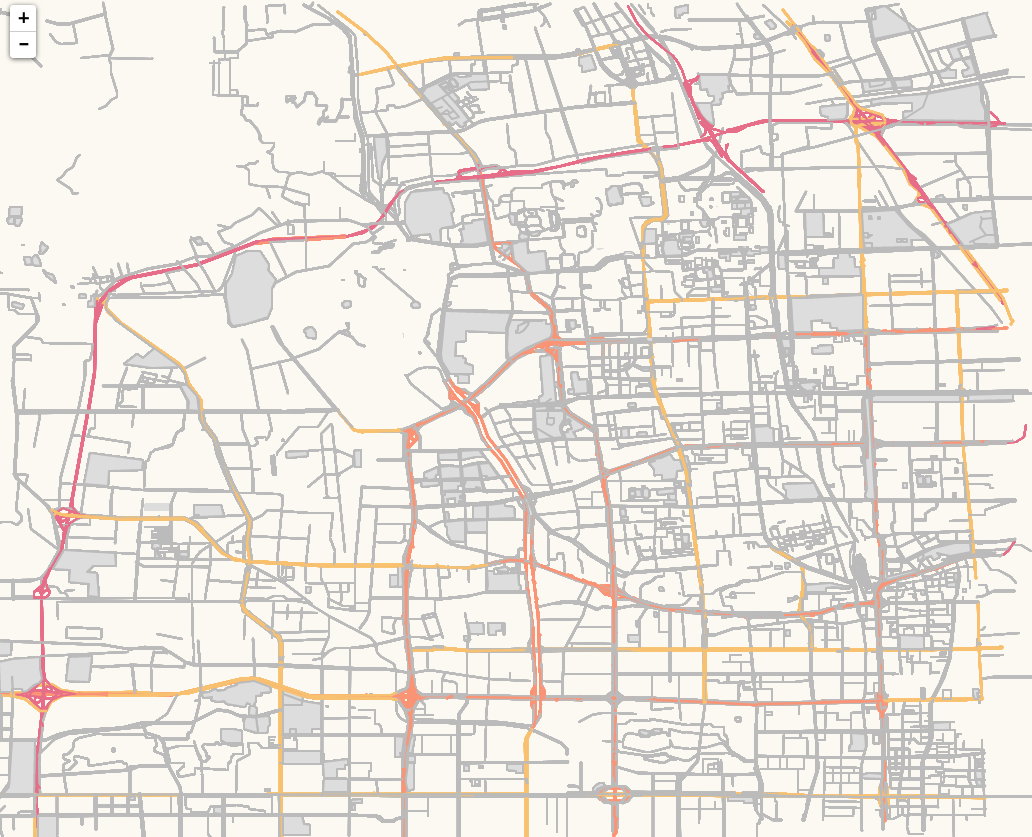
\includegraphics[width=4in]{images/7.png}
    \caption{地图数据上传全图}\label{地图数据上传全图} 
\end{figure}

\begin{figure}[!htb]
    \centering
    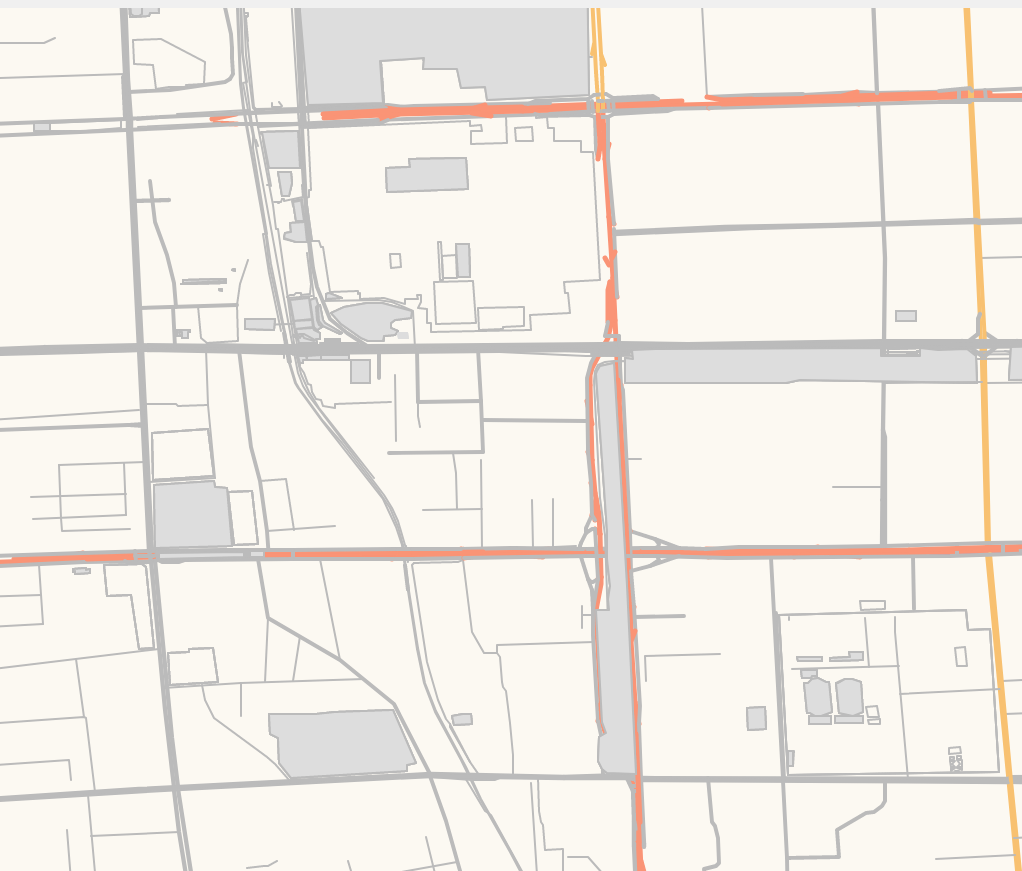
\includegraphics[width=4in]{images/8.png}
    \caption{局部放大图}\label{局部放大图} 
\end{figure}

\subsection{复现车辆位置验证与信誉评估}
车辆位置验证与信誉评估系统,实现了在完成用户验证的基础上为其他使用者提供位置信息和信用评估的数据支持,增强了车载自组网的安全性的同时扩展了应用场景\cite{lposition}。但是,李玮琪调用的地图数据是由openstreetmap提供的矢量地图数据,地图数据安全性得不到保障。本次测试,将李玮琪的工作和地图数据存储和展现结合起来,在完全基于GeoHash编码的GeoHashTile前端进行展示,同时将合约部署至树状区块链上,再次验证树状区块链相关功能的正确性。

车辆位置验证及信誉评估系统主要分为车辆位置采集修正系统和信誉评估系统两个部分\cite{lposition}。车辆位置采集修正系统运行在网页端,获取用户的GPS信息,并根据附近道路实时修正位置,实现与智能合约进行交互,信誉评估系统由只能合约实现并部署在区块链上,负责接收位置采集修正系统的上传的数据,结合已保存的信誉对用户信誉进行更新。

测试流程如下:
\begin{enumerate}
    \item 将信誉评估合约部署至树状区块链上 \\
    由于本文使用的最新的开发环境,重现过程中出现过很多问题,作者对其进行记录,并形成文档,希望对其他人有所帮助。
    \item 将地图显示和该系统结合起来 
    \item 信誉测试路径如图\ref{信誉测试路径}所示
    \begin{figure}[!htb]
        \centering
        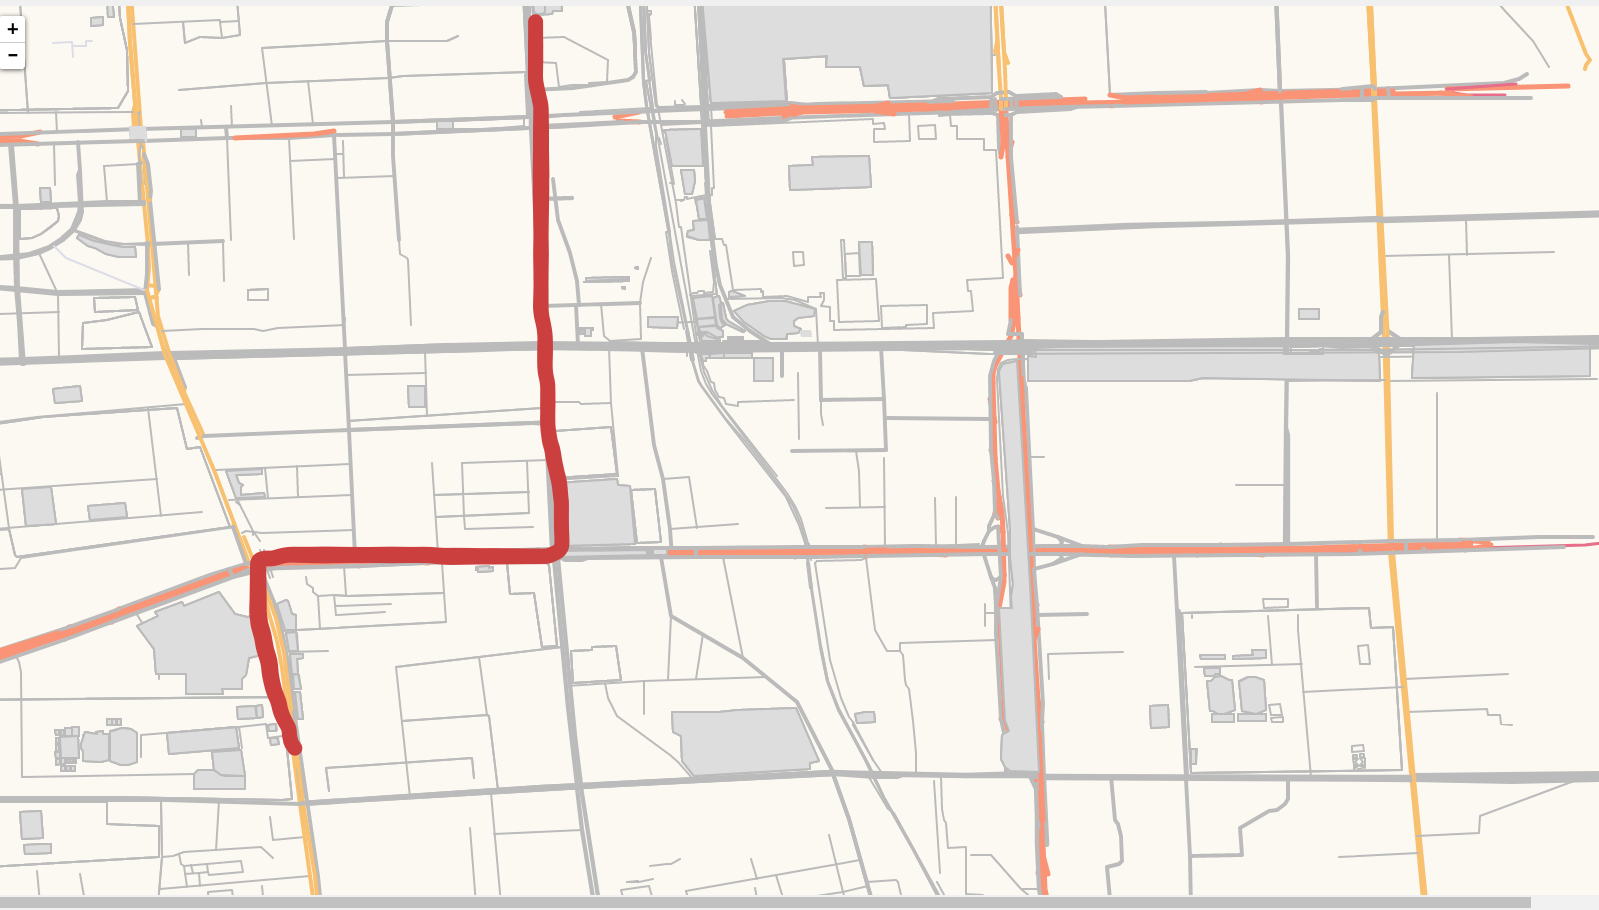
\includegraphics[width=4in]{images/9.png}
        \caption{信誉测试路径}\label{信誉测试路径} 
    \end{figure}

    \item 最终测试结果如图\ref{信誉测试结果}所示
    \begin{figure}[!htb]
        \centering
        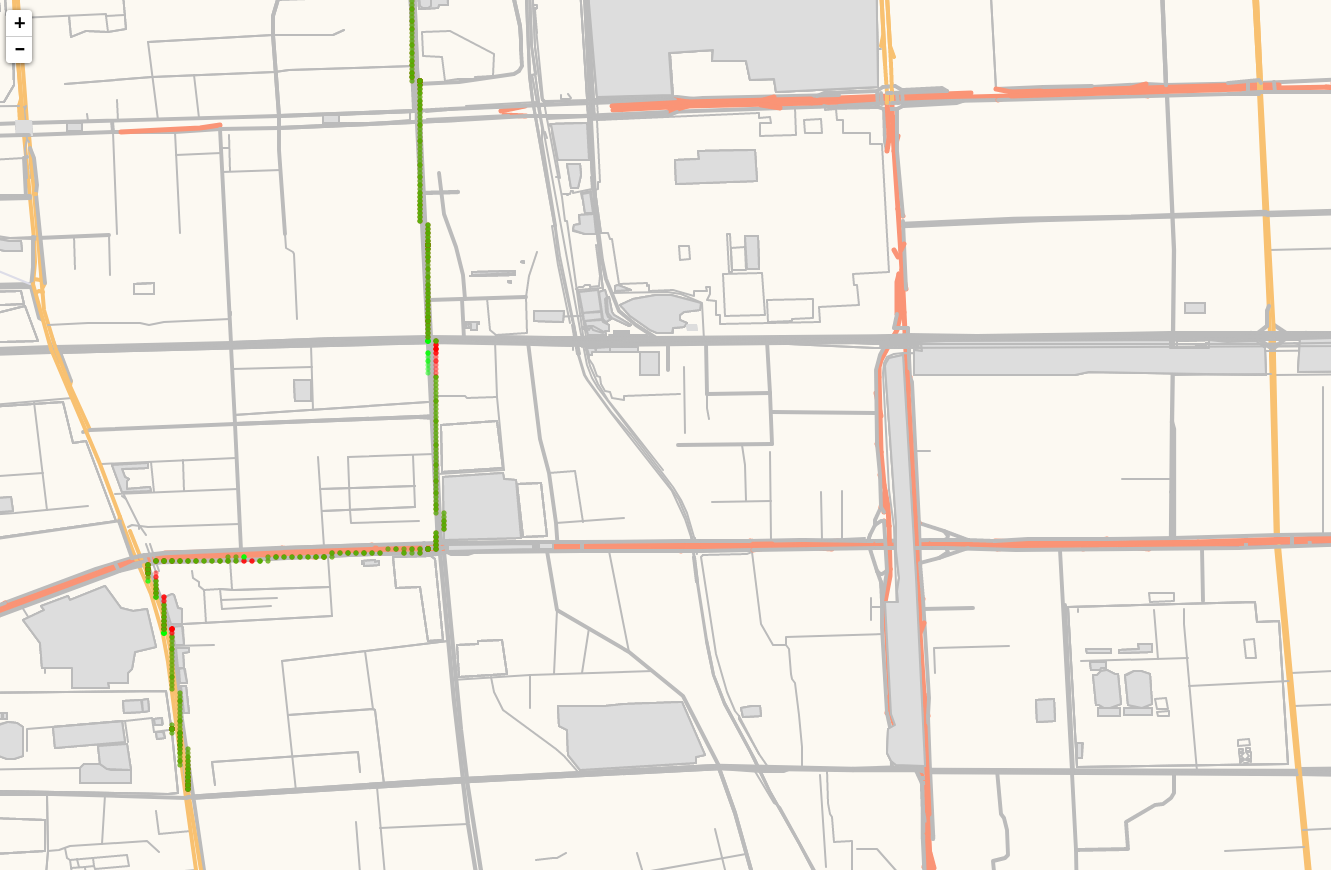
\includegraphics[width=4in]{images/10.png}
        \caption{信誉测试结果}\label{信誉测试结果} 
    \end{figure}
\end{enumerate}

\section{传统区块链合约存储和树状区块链直接存储对比}
此次实验对树状区块链的交易性能进行测试。树状区块链由于本身与地理信息进行绑定,交易时会自动将地理信息存储下来,而传统区块链没有,所以使用智能合约在传统区块链模拟树状区块链的存储状态,对二者效率进行对比,从而评定树状区块链的效率。
\subsection{实验设计思路}
树状区块链会自动维护区域状态树和账户状态树,交易时本身就会存储位置信息。为了在传统区块链上模拟树状区块链的存储量,本次测试需要设计存储合约。

存储合约算法如算法\ref{存储合约}。
\begin{algorithm}[t]
    \caption{存储合约} %算法的名字
    \label{存储合约}
    \begin{algorithmic}[1] %每行显示行号  
        % \Require Array数组,n数组大小  
        \Require from\_account,position,transactionhash,receipt,txttime
        \Function {setInfo}{from\_account,position,transactionhash,receipt,txttime} 
            // 实现存储  
            \State  Onelog.from\_account <- from\_account;
            \State  Onelog.position <- position;
            \State  Onelog.transactionhash <- transactionhash;
            \State  Onelog.recleipt <- receipt;
            \State  Onelog.txttime <-txttime;
            \State  bind\_to\_position(position,from\_account)
        \EndFunction  

        \Function {bind\_to\_position}{position,from\_account}  //实现位置绑定 
            //去重
            \If {CheckDup(from\_account)} 
            {
                \Return
            }
            \Else
                \State position\_area\_accounts[position].num <- position\_area\_accounts[position].num + 1;
                \State position\_area\_accounts[position].account\_list[num] <- from\_account
            \EndIf
        \EndFunction  
        \Function {getInfo\_by\_id}{id}  //通过id查询信息
            \Return {from\_account,position,transactionhash,receipt,txttime}
        \EndFunction  
        \Function {getAccount\_by\_position}{position}  //通过位置查询信息
            \State accounts <- NULL
            \State length <-  position\_area\_accounts[position].num;
            \For {i = 0 -> length}
                \State accounts[i] = position\_area\_accounts[position].account\_list[i]
            \EndFor 
            \Return accounts;
        \EndFunction
    \end{algorithmic}  
\end{algorithm}

本次测试中,传统区块链和树状区块链实际存储数据内容相同,传统区块链由于没有与位置信息进行绑定,所以采用合约的方法进行存储,模拟树状区块链状态,而树状区块链则采用eth直接发送交易,测试算法如算法\ref{测试算法}。
\begin{algorithm}[t]
    \caption{测试算法} %算法的名字
    \label{测试算法}
    \begin{algorithmic}[1] %每行显示行号  
       \State web3绑定
       \State spos1 <- "w1111111111111";
       \State st <- Date();
       \For{i = 0 -> length}
            \State si = i.toString()
            \State subpos <- spos1.substr(0,14-sj.length);
            \State \_position <- subpos+sj;
            \State 合约交易或eth.sendtransaction直接交易
            \State sleep(100);
       \EndFor
       \State 等待区块链存储完毕
       \State se <- Date()-st
       \State 打印结果
    \end{algorithmic}  
\end{algorithm}
\subsection{实验结果}
\begin{table}[!ht]
    \centering
    \caption{测试结果}
    \label{测试结果}
    \begin{tabular}{*{4}{>{\centering\arraybackslash}p{3cm}}}
    \hline
           &  存储数据量      & 传统区块链合约存储时间        & 树状区块链直接存储时间      \\ \hline
      1    &  1200条         & 179518ms                    & 179888ms                  \\
      2    &  2400条         & 376738ms                    & 358368ms                  \\
      3    &  6000条         & 952859ms                    & 915299ms                  \\ 
      4    &  12000条        & 1871136ms                   & 1812014ms                  \\
      \hline
      \end{tabular}
  \end{table}

  表\ref{测试结果}中显示,同样的数据量存储,利用智能合约存储至传统区块链中要比树状区块链直接存储的时间长,而且,这种趋势将随着这数据量的增多而愈发明显。根据上述数据对比,树状区块链对于信息存储效率要比传统区块链好,且树状区块链自身与位置信息绑定,又提供区域查询等更多位置信息查询功能,要比传统区块链更适应于车载自组网。

  \section{小结}
本章中,在树状区块链和地图存储的基础上复现了李玮琪的车辆位置验证与信誉评估的工作,验证了树状区块链的正确性。最后,对树状区块链存储方面进行了性能测试,可以明显发现,随着发送数量的增加,树状区块链本身具备地理信息的优势逐渐增大,存储速率要比传统区块链有所加快,并随着数据量的增加而越发明显,树状区块链在存储同样信息的同时,又保证区域绑定、区域查询功能,且能够自动维护区域状态树以及账户状态树,其功能性更加强大。